\section{Múltiples bibliografías}

La mayoría de los documentos tienen una sola bibligrafía, pero a veces se requieren varias. 

\subsection{Separar la bibliografía}

Es fácil poder separar la bibliografía según el tipo de documento que se esté listando, por ejemplo: libros, artículos, tesis. Para poder lograrlo, hay que generar varias instancias del comando \verb|\printbibliography[option]| con distintas opciones, indicadas en la sección anterior. 

Por ejemplo, podemos separar la biliografía en una lista de libros y en otra de artículos de la siguiente manera:
\begin{lstlisting}
	\printbibliography[type=book,title=Libros]
	\printbibliography[type=misc,title=Paginas web]
\end{lstlisting}

El código anterior genera las siguientes listas de referencias bibliográficas:
\printbibliography[type=book,title=Libros]
\printbibliography[type=misc,title=Páginas web]

Notar que solamente aparecen las referencias que han sido mencionadas en el documento y no todas las que se encuentran en el archivo \verb|.bib|.

\subsection{Una bibliografía por capítulo}
Bib\LaTeX permite tener una lista de referencias bibliográficas separada por capítulo o cualquier parte del documento. Para poder hacerlo, hay que crear el entorno \verb|\begin{refsection}| \verb|.. \end{refsection}| y colocar el texto o parte del documento que se quiera dentro de éste entorno. Al colocar el comando \verb|\printbibliography[]| en ese entorno, se genera la lista de referencias bibliográficas para ese caso. \\


A modo de ejemplo, veamos el siguiente código:
\begin{lstlisting}
	\documentclass[a4paper,12pt]{article}
	
	\usepackage[T1]{fontenc}
	\usepackage[utf8]{inputenc}
	\usepackage[english,spanish,mexico]{babel}
	\usepackage{palatino}
	\usepackage[backend=biber,style=apa,sortcites,natbib=true]{biblatex}
	\urlstyle{sf} 
	\DeclareLanguageMapping{spanish}{spanish-apa}  
	
	\addbibresource{biblio_1.bib}
	
	\begin{document}
		\section{Primer parte}
		\begin{refsection}
			Esta es la parte inicial documento, con \cite{guia1}.
			\printbibliography[heading=subbibliography]
		\end{refsection}
		
		\section{Segunda parte}
		\begin{refsection}
			Esta es la parte final del documento, con \cite{biber}.
			\printbibliography[heading=subbibliography]
		\end{refsection}
	\end{document}
\end{lstlisting}

En la figura siguiente se puede ver el resultado obtenido del código presentado. Se utiliza la opción \verb|heading=subbibliography| en este caso, para que el formato del título sea más pequeño que el de una sección.

\begin{figure}[h]
	\centering
	\fbox{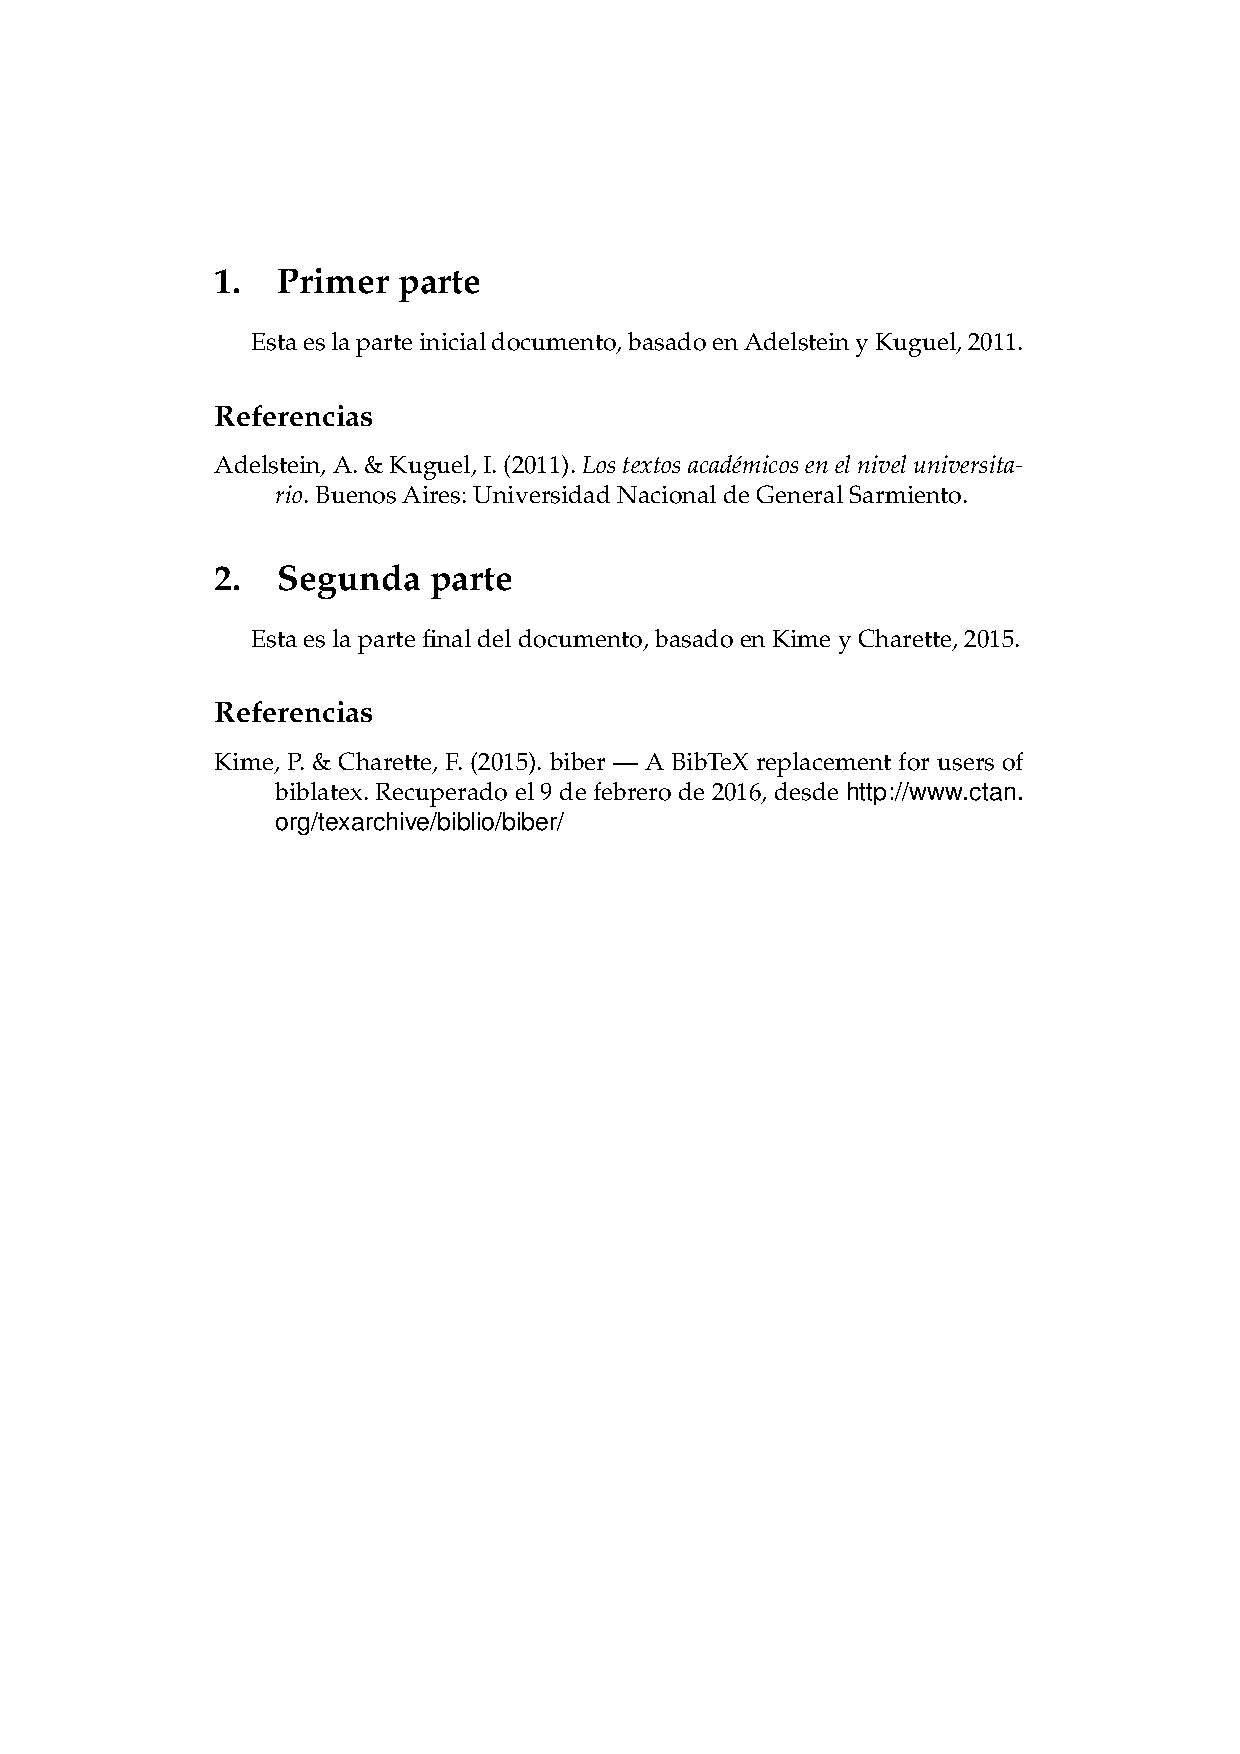
\includegraphics[width=0.8\linewidth]{Ejemplo_split_biblio}}
	\caption{Ejemplo de una bilbiografía por sección del documento.}
	\label{fig:ejemplosplitbiblio}
\end{figure}

Una variante a lo anterior es imprimir todas las listas de referencias bibliográficas por sección al final del documento. Esto se hace colocando al final del documento el comando de cada bibliografía a imprimir, en donde cada \verb|refsection| se numera en orden de aparición. Por lo tanto, el código a colocar al final del documento es:
\begin{lstlisting}
	...
	\printbibliography[section=1,title=Referencias de primer parte]
	\printbibliography[section=2,title=Referencias de segunda parte]
\end{document}
\end{lstlisting}

\begin{figure}[h]
\centering
\fbox{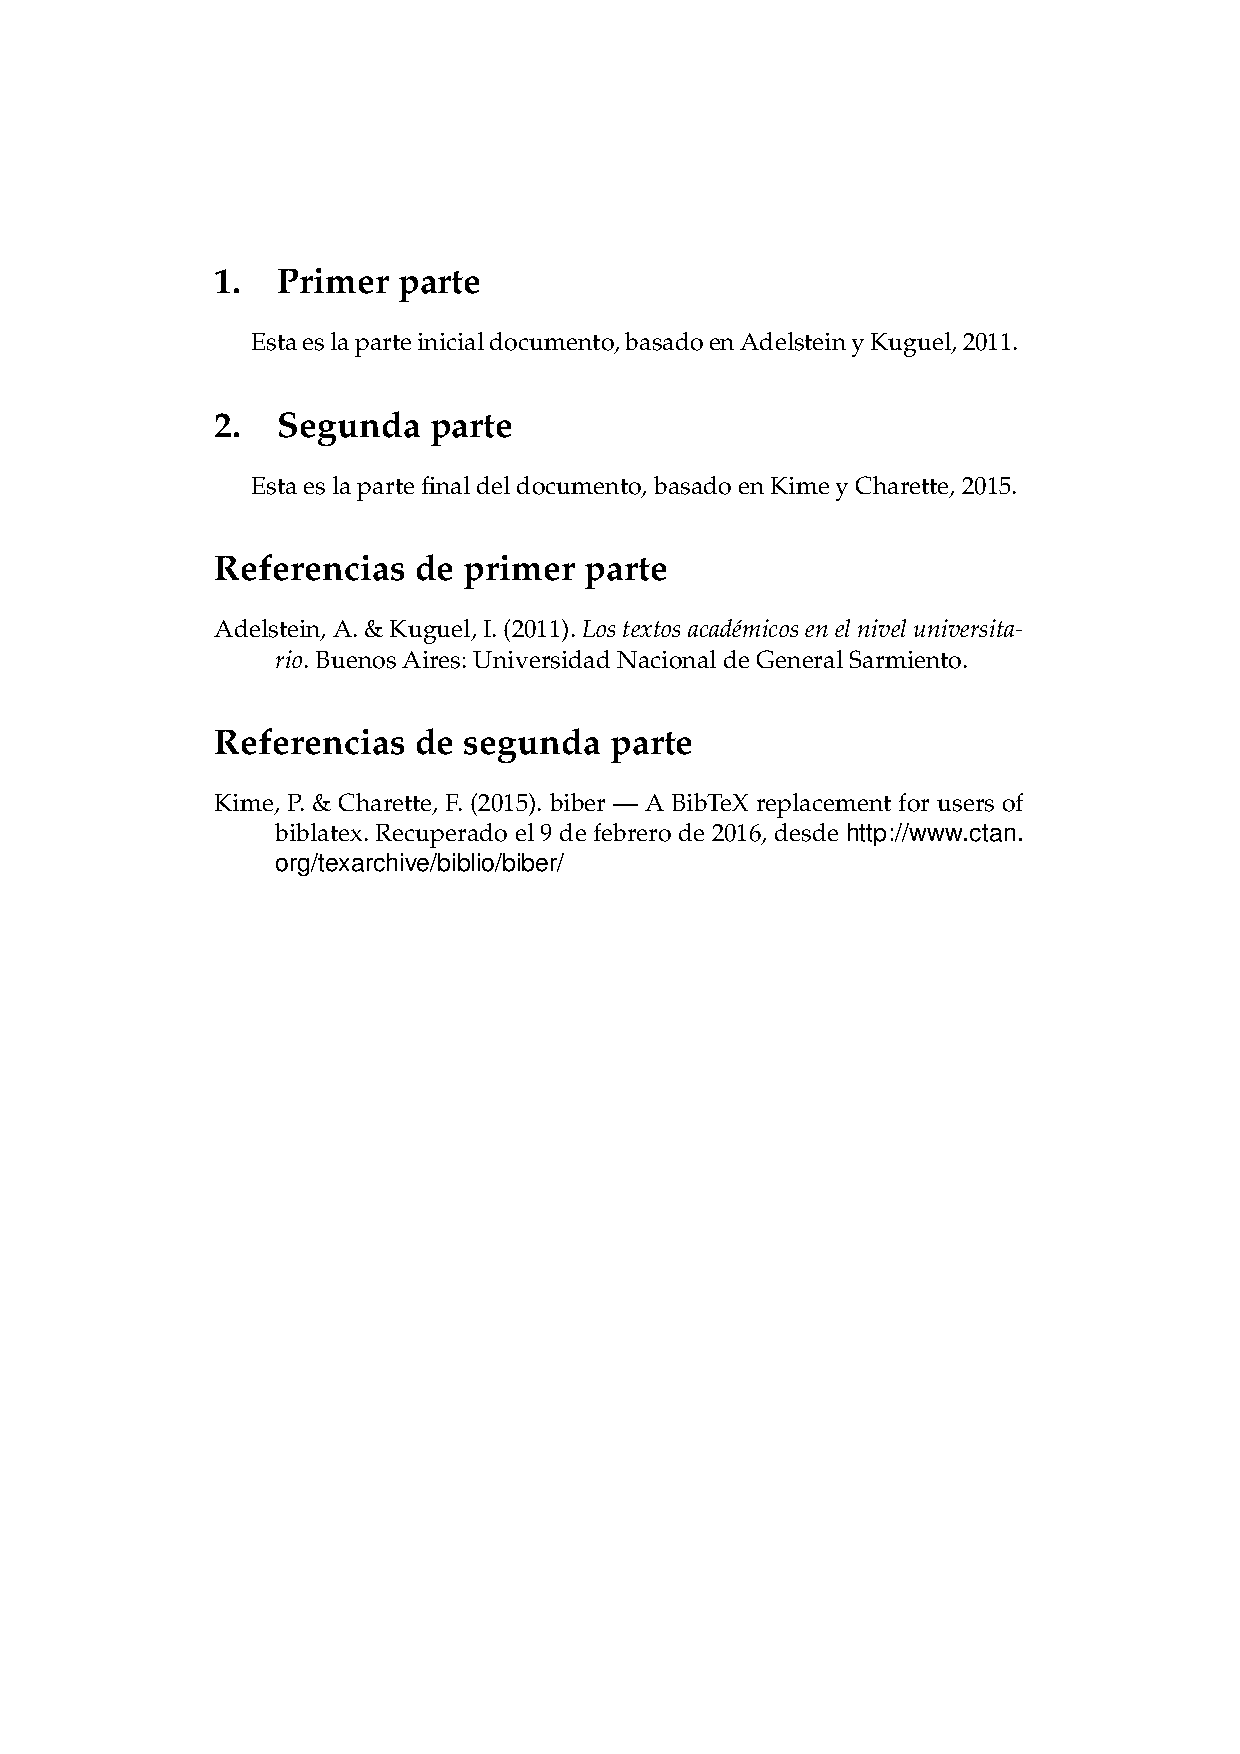
\includegraphics[width=0.8\linewidth]{Ejemplo_split_biblio_2}}
\caption{Ejemplo de una bilbiografía por sección al final del documento.}
\label{fig:ejemplosplitbiblio}
\end{figure}
\newpage

